
\documentclass[./Thick_TQFTs_and_Quantum_Information.tex]{subfiles}

\begin{document}

\section{Paths for Parallel Transport}

In order to obtain linear maps by parallel transport on manifolds, we need
additional structure on top of connections. These are collections of paths on
manifolds along which we will parallel transport vectors in the fibres of a
bundle with connection. We shall now formalize this apparatus in terms of
categories. We will require a notion of graphs on manifolds whose vertices are
points, possibly repeated, on the manifold and whose edges are paths on the
manifold.


\subsection{Graphs Encoding Algebraic Expressions}\label{subsec:alg_graph_exp}

We will now describe a method of encoding expressions involving tensor products,
point-wise algebra products and composition of linear maps $A \to A$ for some
algebra $A$, using directed graphs. As a matter of convention, we will take all
graphs to mean directed acyclic graphs where we do not allow parallel edges or
self-loops, unless stated otherwise. However, we do allow the underlying
undirected graph of any directed graph to be a forest. Given a graph
$G = (V, E)$, we will write $V = V(G)$ and $E = E(G)$. We now see a motivating
example.

\begin{exm}\label{exm:egraph1}
Consider a graph consisting of nine vertices $1, \dots, 9$ with
$V_1 = \set{1, 2}$, $V_2 = \set{3, 4}$, $V_4 = \set{5, 6, 7}$ and
$V_4 = \set{8, 9}$, along with edges:
\[\begin{array}{ccccc}
  (1, 3) &,& (1, 4) &,& (2, 3),\\
  (3, 5) &,& (3, 6) &,& (4, 7),\\
  (5, 8) &,& (6, 9) &,& (7, 9)
\end{array}\]
We visualize this graph as follows:
\[\begin{tikzpicture}[xscale=2,yscale=0.5]
\node at (0, 3) (v1) {1};
\node at (0, 1) (v2) {2};
\node at (1, 3) (v3) {3};
\node at (1, 1) (v4) {4};
\node at (2, 4) (v5) {5};
\node at (2, 2) (v6) {6};
\node at (2, 0) (v7) {7};
\node at (3, 3) (v8) {8};
\node at (3, 1) (v9) {9};
\midarrow{v1}{v3}
\midarrow[0.33]{v1}{v4}
\midarrow[0.33]{v2}{v3}
\midarrow{v3}{v5}
\midarrow{v3}{v6}
\midarrow{v4}{v7}
\midarrow{v5}{v8}
\midarrow{v6}{v9}
\midarrow{v7}{v9}
\end{tikzpicture}\]
Thinking of individual edges in the above graph as mappings $A \to A$ of some
monoid and comonoid $A$ in some monoidal category, we can think of multiple
incoming edges on a vertex -- for example, the incoming edges on $3$ -- as a
multiplication $\cwedge$ of maps and multiple outgoing edges -- for example, the
outgoing edges of $1$ -- as a comultiplication $\cvee$ of maps. Parallel edges,
multiplications or comultiplications with disjoint sources and targets can be
thought of as a tensor product of maps. We can treat a single vertex as an
identity mapping.

We can then modify the graph as follows:
\[\begin{tikzpicture}[xscale=2,yscale=0.75]
\node at (-2, 3) (v1) {1};
\node at (-2, 1) (v2) {2};
\node at (-1, 4) (v33) {3};
\node at (-1, 2) (v44) {4};
\node at (-1, 1) (v22) {2};
\node at (0, 4) (v333) {3};
\node at (0, 2) (v3333) {3};
\node at (0, 1) (v444) {4};
\node at (1, 3) (v3) {3};
\node at (1, 1) (v4) {4};
\node at (2, 4) (v5) {5};
\node at (2, 2) (v6) {6};
\node at (2, 0) (v7) {7};
\node at (3, 3) (v8) {8};
\node at (3, 1) (v9) {9};
\midarrow{v1}{v33}
\midarrow{v1}{v44}
\midarrow{v2}{v22}
\midarrow{v33}{v333}
\midarrow[0.33]{v22}{v3333}
\midarrow[0.33]{v44}{v444}
\midarrow{v333}{v3}
\midarrow{v3333}{v3}
\midarrow{v444}{v4}
\midarrow{v3}{v5}
\midarrow{v3}{v6}
\midarrow{v4}{v7}
\midarrow{v5}{v8}
\midarrow{v6}{v9}
\midarrow{v7}{v9}
\end{tikzpicture}\]
Thinking of edges between copies of the same vertex, which did not originally
exist, as the identity map and crossing edges as a twist operation -- denoted
$\boxtimes$ -- of maps, we can capture the graph into an algebraic expression of
the following form:
\begin{align*}
        & ((5, 8) \tensor ((6, 9) \cwedge (7, 9))) \\
  \circ & ((3, 5) \tensor (3, 6) \tensor (4, 7)) \\
  \circ & (((3, 3) \cvee (3, 3)) \tensor (4, 4)) \\
  \circ & ((3, 3) \tensor ((4, 4) \boxtimes (2, 3))) \\
  \circ & (((1, 3) \cvee (1, 4)) \tensor (2, 2))
\end{align*}

Observe that we have taken a directed acyclic graph and converted it to a
diagram in $\Cob_{2}$ -- the symmetric monoidal category of cobordisms of
dimension $2$. This, in turn, yields an expression involving operations on
endomorphisms of a Frobenius monoid in some monoidal category. However, we
should note that this is just one possible interpretation of the graph above.
\end{exm}

This motivates us to define an algorithm for extracting expressions from a
directed acyclic graph such as the one above.
\begin{alg}[Expression Construction]
Let $G = (V, E)$ be any graph. We make the following modifications to $G$:
\begin{enumerate}
\setlength{\itemsep}{0pt}

\item For each vertex $v$, choose an ordering of the incoming edges of $v$, say
$(u_1, v), \dots, (u_k, v)$ and and ordering of its outgoing edges, say
$(v, w_1), \dots, (v, w_n)$.

\item Let $S(G)$ be the set consisting of vertices with no incoming
edges -- called the source vertices of $G$ -- and $T(G)$, the set consisting of
vertices with no outgoing edges -- called the target vertices of $G$. We then
choose orderings of $S(G)$. Note that $S(G) \cap T(G)$ might be non-empty
because of vertices with no edges, incoming or outgoing.

\item Copy vertices and add edges to make the following modification, where the
incoming edges are in order from the lowest at the top to the highest at the
bottom:
\[\begin{tikzpicture}
\node at (2, 0)     (v) {$v$};
\node at (0, 1)     (u1) {$u_1$};
\node at (0, 0.5)   (u2) {$u_2$};
\node at (0, 0)     (u3) {$u_3$};
\node at (0, -1)    (uk) {$u_k$};
\midarrow{u1}{v}
\midarrow{u2}{v}
\midarrow{u3}{v}
\midarrow{uk}{v}
\draw[thick, loosely dotted] (u3) -- (uk);
\end{tikzpicture}
\qquad
\begin{tikzpicture}
\node at (0, 1)   (TOP)     {};
\node at (0, 0)   (TO)      {$\Longrightarrow$};
\node at (0, -1)  (BOTTOM)  {};
\end{tikzpicture}
\qquad
\begin{tikzpicture}
\node at (4, -1)     (v) {$v$};
\node at (0, 1)     (u1) {$u_1$};
\node at (0, 0.5)   (u2) {$u_2$};
\node at (0, 0)     (u3) {$u_3$};
\node at (0, -1)    (uk) {$u_k$};
\node at (1, 0.5) (a)  {$v$};
\node at (2, 0)   (b)  {$v$};
\midarrow{u1}{a}
\midarrow{u2}{a}
\midarrow{a}{b}
\midarrow{u3}{b}
\draw[thick, loosely dotted] (b) -- (v);
\draw[thick, loosely dotted] (u3)   -- (uk);
\midarrow{uk}{v};
\end{tikzpicture}
\]

\item Copy vertices and edges to make the following modification similar to the
previous step:
\[
\begin{tikzpicture}
\node at (-2, 0)     (v) {$v$};
\node at (0, 1)     (w1) {$w_1$};
\node at (0, 0.5)   (w2) {$w_2$};
\node at (0, 0)     (w3) {$w_3$};
\node at (0, -1)    (wk) {$w_k$};
\midarrow{v}{w1}
\midarrow{v}{w2}
\midarrow{v}{w3}
\midarrow{v}{wk}
\draw[thick, loosely dotted] (u3) -- (uk);
\end{tikzpicture}
\qquad
\begin{tikzpicture}
\node at (0, 1)   (TOP)     {};
\node at (0, 0)   (TO)      {$\Longrightarrow$};
\node at (0, -1)  (BOTTOM)  {};
\end{tikzpicture}
\qquad
\begin{tikzpicture}
\node at (-4, -1)   (v)  {$v$};
\node at (0, 1)     (w1) {$w_1$};
\node at (0, 0.5)   (w2) {$w_2$};
\node at (0, 0)     (w3) {$w_3$};
\node at (0, -1)    (wk) {$w_k$};
\node at (-1, 0.5) (a)  {$v$};
\node at (-2, 0)   (b)  {$v$};
\midarrow{a}{w1}
\midarrow{a}{w2}
\midarrow{b}{a}
\midarrow{b}{w3}
\draw[thick, loosely dotted] (b) -- (v);
\draw[thick, loosely dotted] (w3)   -- (wk);
\midarrow{v}{wk};
\end{tikzpicture}
\]

\item At this point, every vertex has both indegree and outdegree at most $2$.
The chosen edge orderings induces a local geometric orientation -- in an
informal sense -- on the graph. By this we mean, that this allows us to
distinguish the following diagrams in a precise sense:
\[
\begin{tikzpicture}
\node at (0, 0) (u) {$u$};
\node at (2, 0.5) (v) {$v$};
\node at (2, -0.5) (w) {$w$};
\midarrow{u}{v}
\midarrow{u}{w}
\end{tikzpicture}
\qquad
\qquad
\begin{tikzpicture}
\node at (0, 0) (u) {$u$};
\node at (2, -0.5) (v) {$v$};
\node at (2, 0.5) (w) {$w$};
\midarrow{u}{v}
\midarrow{u}{w}
\end{tikzpicture}
\]

The distinction is that if we take $(u, v) < (u, w)$ in the left picture, say,
then we can take $(u, v) > (u, w)$ in the right picture.
Then, for every edge that is shared between a ``multiplication'' and a
``comultiplication'', considering the edge orderings chosen before, we have the
following possibilities for common edges and we make the modifications shown:
\[
\begin{tikzpicture}
\node at (0, 2) (u) {$u$};
\node at (2, 2) (v) {$v$};
\node at (0, 0) (w) {$w$};
\node at (2, 0) (x) {$x$};
\midarrow{u}{v}
\midarrow{u}{x}
\midarrow{w}{x}
\end{tikzpicture}
\qquad
\begin{tikzpicture}
\node at (0, 1)   (TOP)     {};
\node at (0, 0)   (TO)      {$\Longrightarrow$};
\node at (0, -1)  (BOTTOM)  {};
\end{tikzpicture}
\qquad
\begin{tikzpicture}
\node at (0, 2) (u) {$u$};
\node at (2, 2) (a) {$v$};
\node at (4, 2) (v) {$v$};
\node at (2, 1) (b) {$x$};
\node at (0, 0) (w) {$w$};
\node at (2, 0) (c) {$w$};
\node at (4, 0) (x) {$x$};
\midarrow{u}{a}
\midarrow{a}{v}
\midarrow{u}{b}
\midarrow{b}{x}
\midarrow{w}{c}
\midarrow{c}{x}
\end{tikzpicture}
\]
\[
\begin{tikzpicture}
\node at (0, 0) (u) {$u$};
\node at (1, 2) (v) {$v$};
\node at (2, 0) (w) {$w$};
\midarrow{u}{v}
\midarrow{v}{w}
\midarrow{u}{w}
\end{tikzpicture}
\qquad
\begin{tikzpicture}
\node at (0, 1)   (TOP)     {};
\node at (0, 0)   (TO)      {$\Longrightarrow$};
\node at (0, -1)  (BOTTOM)  {};
\end{tikzpicture}
\qquad
\begin{tikzpicture}
\node at (0, 1) (u) {$u$};
\node at (2, 2) (v) {$v$};
\node at (2, 0) (a) {$w$};
\node at (4, 1) (w) {$w$};
\midarrow{u}{v}
\midarrow{u}{a}
\midarrow{v}{w}
\midarrow{a}{w}
\end{tikzpicture}
\]

\[
\begin{tikzpicture}
\node at (0, 2) (u) {$u$};
\node at (2, 2) (v) {$v$};
\node at (0, 0) (w) {$w$};
\node at (2, 0) (x) {$x$};
\midarrow{u}{v}
\midarrow[0.33]{w}{v}
\midarrow[0.33]{u}{x}
\end{tikzpicture}
\qquad
\begin{tikzpicture}
\node at (0, 1)   (TOP)     {};
\node at (0, 0)   (TO)      {$\Longrightarrow$};
\node at (0, -1)  (BOTTOM)  {};
\end{tikzpicture}
\qquad
\begin{tikzpicture}
\node at (0, 2) (u) {$u$};
\node at (2, 2) (a) {$v$};
\node at (4, 2) (aa) {$v$};
\node at (6, 2) (v) {$v$};
\node at (2, 1) (b) {$x$};
\node at (4, 1) (bb) {$w$};
\node at (0, 0) (w) {$w$};
\node at (2, 0) (c) {$w$};
\node at (4, 0) (cc) {$x$};
\node at (6, 0) (x) {$x$};
\midarrow{u}{a}
\midarrow{u}{b}
\midarrow{w}{c}
\midarrow{a}{aa}
\midarrow[0.33]{b}{cc}
\midarrow[0.33]{c}{bb}
\midarrow{aa}{v}
\midarrow{bb}{v}
\midarrow{cc}{x}
\end{tikzpicture}
\]

We also make the modifications obtained from the rotations of the above diagrams
about a horizontal edge. After these modifications have been applied, there are
no edges shared between ``multiplications'' and ``comultiplications''.

\item Noting that $G$ is acyclic even after the modifications, we construct a
level ordering of $G$ inductively as follows:
\begin{enmrt}
\li Let $V_1$ be the set of vertices with no incoming edges -- i.e.,
$V_1 := S(G)$
\li Let $V_{k + 1}$ be the set of vertices in
$G \setminus (V_1 \cup \cdots \cup V_k)$ with incoming edges only from
$V_1, \dots, V_k$, or with no incoming edges.
\end{enmrt}
We note that the ordering on $S(G) = V_1$ induces an ordering of $V_2$ as
follows. Let $S(G)$ be ordered as $u_1, \dots, u_n$. Let the ordering of the
outgoing edges of $u_i$ be $(u_i, v_{i, 1}), \dots, (u_i, v_{i, k_i})$. We let
$v_i := v_{1, i}$ for $1 \leq i \leq k_1$. For $1 \leq j < n$,
$k_j < i \leq k_{j + 1}$, we let $v_i := v_{j + 1, i}$. Then, the $v_i$ are an
ordering of $V_2$. We can repeat this process with $V_2$ in place of $S(G)$ and
so on to obtain an ordering for each level. By construction, we have the
following corollary:

\begin{cor}\label{cor:lvltolvl}
Let $G$ be an expression graph with induced level ordering
$V_1, V_2, \dots, V_k$. Then for each $i \in \set{2, \dots, k}$ and each
$v \in V_i$ that is not edgeless, there is an edge $(u, v)$ with
$u \in V_{i - 1}$.
\end{cor}

\begin{rmk}
This level ordering algorithm works on any graph -- in particular, on $G$
before the modifications. We will need this construction on arbitrary graphs
later on.
\end{rmk}

\begin{rmk}
The vertices with no edges, incoming or outgoing, are always in the first level.
We will call these vertices edgeless vertices. However, vertices with no
outgoing edges need not always be in the last level.
\end{rmk}

\item\label{alg:edgeless}
Consider the vertices with no outgoing edges but not at the last level. For each
such vertex $u$ in $V_i$, we add a copy $u'$, to $V_{i + 1}$. Its insertion
order needs to be made precise. Call the vertices in $V_{i + 1}$ with an
incoming edge from some vertex above $u \in V_{i}$, the vertices above $u$ in
$V_{i + 1}$. Similarly, call the vertices in $V_{i + 1}$ with no incomoing edges
from $u$ or a vertex above $u \in V_i$, the vertices below $u$ in $V_{i + 1}$.
A copy of $u$, say $u'$, is inserted
in the position right after the vertices above $u$ and before the vertices below
$u$ in $V_{i + 1}$. We then add in the edge $(u, u')$. We continue this process
with $V_{i + 1}$ in place of $V_i$ and so on until, there is a copy
of $u$ in each level after $V_i$ with a path connecting them.

\begin{rmk}
Each vertex without any edges, incoming or outgoing, are also copied in this
way, noting that these vertices are placed in the first level during the level
ordering. We will call these vertices edgeless vertices.
\end{rmk}

\item For each level skipping edge $(u, v)$ -- that is, with $u \in V_k$ and
$v \in V_{k'}$ for some $k' > k + 1$ -- we insert a copy of $u$ in $V_{i}$ for
each $k < i < k'$ in positions similar to the insertions in the last step. We
call this copy $u'$. We then and add an edge $(u, u')$. We repeat this with
$V_{i + 1}$ in place of $V_{i}$ and $u'$ in place of $u$. After this process
completes, we delete the edge $(u, v)$. After we complete this process for every
level-skipping edge, level skipping edges are replaced by paths connecting the
source vertex to the target vertex of these edges.

\item Observe that we can now identify the graph $G$ with a cobordism in
$\Cob_2$ from $|S(G)|$ copies of $S^1$ to $|T(G)|$ copies of $S^1$! The
identifications of the generating structures are the obvious ones:
\[
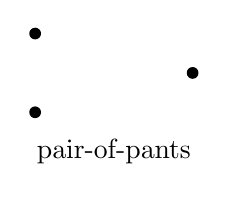
\begin{tikzpicture}
\node[circle, fill, inner sep=1.5pt] at (0, 0) (u) {};
\node[circle, fill, inner sep=1.5pt] at (-2, 0.5) (v) {};
\node[circle, fill, inner sep=1.5pt] at (-2, -0.5) (w) {};
\midarrow{v}{u}
\midarrow{w}{u}
\node at (-1, -1) (lbl) {pair-of-pants};
\end{tikzpicture}
\qquad
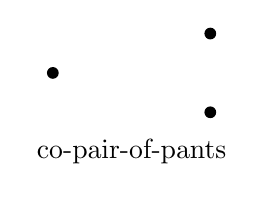
\begin{tikzpicture}
\node[circle, fill, inner sep=1.5pt] at (0, 0) (u) {};
\node[circle, fill, inner sep=1.5pt] at (2, -0.5) (v) {};
\node[circle, fill, inner sep=1.5pt] at (2, 0.5) (w) {};
\midarrow{u}{v}
\midarrow{u}{w}
\node at (1, -1) (lbl) {co-pair-of-pants};
\end{tikzpicture}
\qquad
\begin{tikzpicture}
\node[circle, fill, inner sep=1.5pt] at (0, 0) (u) {};
\node at (2, -0.5) (v) {};
\node at (2, 0.5) (w) {};
\node[circle, fill, inner sep=1.5pt] at (2, 0) (x) {};
\midarrow{u}{x}
\node at (1, -1) (lbl) {cylinder};
\end{tikzpicture}
\]

Note that the cap or cup were not used. This, then, directly yields an
expression of the original graph $G$ similar to the example.

\end{enumerate}
\end{alg}

\begin{defn}[Expression of a Graph]
Given a graph $G$, the expression resulting from the algorithm above is called
an expression of $G$ and denoted $\Exp{G}$.
\end{defn}

\begin{rmk}
Note that an expression of a graph is by no means unique -- we made a large
number of arbitrary choices in our process.
\end{rmk}

\begin{rmk} We also note that we did not specify how to handle ``crossings'' of
edges but it is not difficult to see that ``crossing'' makes precise sense when
we specify the edge orderings and the ordering of the source of a graph. Once we
execute the algorithm above, we can handle crossings in the same way we handle
then when drawing cobordisms in $\Cob_2$.
\end{rmk}

Even though we made many choices in the above algorithm, the only
choices that cannot be thought of as canonical in any way are the chosen edge
orderings and the ordering of the source vertices. We are thus motivated to make
the following definition.

\begin{defn}[Expression Graph]
A graph with a chosen edge ordering and a chosen ordering of its source vertices
is called an expression graph.
\end{defn}

Thus, given an expression graph, we have an algorithm to extract its expression
consistently as long as we keep the other choices in the above algorithm fixed.
We will later see that $\Exp{G}$ is functorial in a suitable sense.




\subsection{Morphisms of Expression Graphs}

It is of interest to define morphisms of expression graphs. They will be
necessary to define interesting constructions on expression graphs later on.

\begin{defn}[Expression Homomorphism]
An expression graph homomorphism or expression homomorphism is a graph
homomorphism $f : G \to H$ between expression graphs such that $f(S(G))$ is
contained in some level set $L$ in $H$, $f$ preserves the ordering of $S(G)$ in
$L$ and $f$ preserves the edge orderings for each vertex.
\end{defn}

We then note some useful facts concerning level orderings and expression
isomorphisms. First, every expression graph $G$ has a level ordering as
described in the algorithm in \S\ref{subsec:alg_graph_exp} so that the vertex
set is a disjoint union of the levels. Then, we have a level function $l_G$ for
$G$ which assigns to each vertex $v$ the integer $n$ for which $v$ is in the
$n$--th level set.

\begin{lem}\label{thm:expiso_lvlpres}
Expression isomorphisms $f : G \to H$ are level preserving, i.e.
\[
  l_G(v) = l_H(f(v))
\]
\end{lem}
\begin{proof}
Let
$\set{V_i}_{i = 1}^{N}$ and
$\set{W_j}_{i = 1}^{M}$ be the level sets of $G$ and $H$
respectively. Let $v \in V_k$ for some $1 \leq k \leq N$.
By corollary \ref{cor:lvltolvl}, there is a path $v_1, \dots, v_k = v$ with each
$v_i \in V_i$. Then, there is a path $f(v_1), \dots, f(v_k) = f(v)$ in $H$ with
$l_H(f(v_{i})) < l_H(f(v_{i + 1}))$ (since edges only go forward in levels) and
$l_H(f(v_1)) \geq 1$. Hence, by extending this path in $H$ backwards to $W_1$,
we have that $l_H(f(v)) \geq l_G(v)$.
On the other hand, let $f(v) \in W_m$ so that there is
a path $w_1, \dots, w_m$ in $H$ with each $w_i \in W_i$. Using $f^{-1}$ on this
path and a similar argument as the one before, we can show that
$l_H(f(v)) \leq l_G(v)$.
\end{proof}

\begin{cor}
For any expression isomorphism $f : G \to H$, if $V_i$ is the $i$--th level set
in $G$, then $f(V_i)$ is the $i$--th level set in $H$.
\end{cor}
\begin{proof}
Let $W_i$ be the $i$--th level set of $H$. Then, by the previous lemma
$f(V_i) \subset W_i$. Again, using $f^{-1}$ in place of $f$ and $W_i$ in place
of $V_i$, we have
$f^{-1}(W_i) \subset V_i \implies W_i \subset f(V_i)$. Hence, $f(V_i) = W_i$.
\end{proof}

\begin{lem}
Expression isomorphisms $f : G \to H$ are order-preserving on levels, i.e.
\[
  u \leq v \iff f(u) \leq f(g)
\]
\end{lem}
\begin{proof}
Let $u, v$ be in the same level set in $G$ and $u \leq v$. We proceed by
induction on $l_G(u) = l_G(v)$. When $l_G(u) = l_G(v) = 1$, then
$f(u) \leq f(v)$, by definition. The other direction is obtained similarly with
$f^{-1}$ in place of $f$.

Let $l_G(u) = l_G(v) = k + 1$. By the construction of level sets and their
ordering given in the expression construction algorithm, there exist
$u', v' \in V(G)$ such that the following hold:
\begin{enmrt}
\li $l_G(u') = l_G(v') = k$
\li $u' \leq v'$
\li there are edges $(u', u)$ and $(v' v)$
\li there are no edges $(u'', u)$ or $(v'', v)$ with $u'' < u'$ or $v'' < u'$
\li if $u' = v'$, $(u', u) \leq (v', v)$
\end{enmrt}
By the previous corollary, $l_H(f(u')) = l_H(f(v')) = k$.
If there is an $x < f(u')$ or a $y < f(v')$ in $V(H)$ with edges
$(x, f(u'))$ or $(y, f(v'))$, then by induction, $f^{-1}(x) < u'$ or
$f^{-1}(y) < v'$ with some edge $(f^{-1}(x), u)$ or $(f^{-1}(y), v)$,
contradicting the conditions on $u'$ and $v'$. Thus, the edges $(f(u'), f(u))$
and $(f(v'), f(v))$ ensure that $f(u) \leq f(v)$. The other direction is again
obtained similarly by replacing $f$ with $f^{-1}$.
\end{proof}

\begin{cor}\label{cor:expiso_unique}
Expression isomorphisms $f : G \to H$ are unique.
\end{cor}
\begin{proof}
Let $g : G \to H$ be another expression isomorphism. Then both $f$ and $g$
restrict to order-preserving bijections on the finite level sets and hence must
agree on the level sets. Thus, $f$ and $g$ agree on $G$.
\end{proof}

In light of the last corollary, it is reasonable to consider expression graphs
up to expression isomorphisms from this point onwards. We will next define some
useful constructs on expression graphs that will facilitate our desired notion
of TQFTs.




\subsection{Constructs on Expression Graphs}

Consider expression graphs $G$ and $H$. We can take the disjoint unions of their
vertex and edge sets. It is clear that the edge orderings of the vertices of
$G$ and $H$ collectively provide an edge ordering for every vertex of
$G \amalg H$. We observe that $S(G \amalg H) = S(G) \amalg S(H)$ so that the
orderings of $S(G)$ and $S(H)$ provide an ordering of $S(G \amalg H)$, where the
vertices of $G$ come before those of $H$. The empty graph is an expression and
hence acts as a unit for the disjoint union operation. It is easy to see that
the associators and unitors for the coproduct in the category of sets are
expression isomorphisms.

We then proceed to define a gluing of expression graphs. For an expression
graph $G$, $S(G)$ without any edges is itself an expression graph.
The edgeless vertices are in both $S(G)$ and $T(G)$. Since $S(G)$ is also the
first level of $G$, $S(G)$ is ordered, by definition. We then observe that
$T(G)$ is the union of the last level and the set of edgeless vertices. Thus,
using a method similar to point \ref{alg:edgeless} in the algorithm given in
\S\ref{subsec:alg_graph_exp}, we have an induced ordering of $T(G)$, so that
$T(G)$ is also an expression graph without any edges.
There are obvious order-preserving expression homomorphisms
$S(G) \hto G \hot T(G)$ that are isomorphisms onto their images. We note
that if there is a an expression isomorphism $\psi : S(H) \to T(G)$ for
expression graphs $G$ and $H$, then $\psi$ is unique by \ref{cor:expiso_unique}.
This allows us to define the following notion of gluing.

\begin{defn}[Gluing of Expression Graphs]
Let $G$ and $H$ be expression graphs such that there is a unique expression
isomorphism
\[
  \psi_{G, H} : S(H) \to T(G)
\]
Then, we say that $G$ and $H$ are gluable at $S(H) \cong T(G)$. We define the
pushout of the following span in $\Set$ to be the gluing $H * G$ of graphs.
\[
  H \hot S(H) \to[\phi] T(G) \hto G
\]
\end{defn}

\begin{thm}
Gluings $H * G$ of expression graphs $G$ and $H$ at $S(H) \cong T(G)$ are
expression graphs.
\end{thm}
\begin{proof}
First we show that $S(H * G) = S(G)$. If $v \in S(H * G) \setminus S(G)$, then
$v$ has an incoming edge in $G$ and since gluing does not delete edges, $v$ has
an incoming edge in $H * G$, so that $v \not\in S(H * G)$. Thus,
$S(H * G) \subseteq S(G)$. If $v \in S(G)$, then $v$ has no incoming edges in
$G$. It is clear that gluing cannot introduce incoming edges to the source
vertices of $G$ so that $S(G) \subset S(H * G)$. Thus, $H * G$ also inherits the
ordering of its source vertices from $G$.

We observe that only the vertices in $T(G)$ receive new edges and these are all
outgoing while the vertices in $T(G)$ have no outgoing edges in $G$. Thus,
$H * G$ inherits edge orderings unambiguously from $G$ and $H$ collectively.
Therefore, $H * G$ is an expression graph.
\end{proof}

\begin{exm}\label{exm:expression_gluing}
Consider $G$ from example \ref{exm:egraph1} and $H$ as follows:
\[\begin{tikzpicture}[xscale=2,yscale=0.75]
\node at (3, 3) (v10) {$10$};
\node at (3, 1) (v11) {$11$};
\node at (4, 3) (v12) {$12$};
\node at (4, 1) (v13) {$13$};
\node at (5, 4) (v14) {$14$};
\node at (5, 2) (v15) {$15$};
\node at (5, 0) (v16) {$16$};
\midarrow[0.33]{v8}{v13}
\midarrow[0.33]{v9}{v12}
\midarrow{v8}{v14}
\midarrow{v12}{v14}
\midarrow{v12}{v15}
\midarrow{v13}{v15}
\midarrow{v13}{v16}
\end{tikzpicture}\]
We have the following diagram of $H * G$:
\[\begin{tikzpicture}[xscale=2,yscale=0.75]
\node at (0, 3) (v1) {$1$};
\node at (0, 1) (v2) {$2$};
\node at (1, 3) (v3) {$3$};
\node at (1, 1) (v4) {$4$};
\node at (2, 4) (v5) {$5$};
\node at (2, 2) (v6) {$6$};
\node at (2, 0) (v7) {$7$};
\node at (3, 3) (v8) {$8 \cong 10$};
\node at (3, 1) (v9) {$9 \cong 11$};
\node at (4, 3) (v12) {$12$};
\node at (4, 1) (v13) {$13$};
\node at (5, 4) (v14) {$14$};
\node at (5, 2) (v15) {$15$};
\node at (5, 0) (v16) {$16$};
\midarrow{v1}{v3}
\midarrow[0.33]{v1}{v4}
\midarrow[0.33]{v2}{v3}
\midarrow{v3}{v5}
\midarrow{v3}{v6}
\midarrow{v4}{v7}
\midarrow{v5}{v8}
\midarrow{v6}{v9}
\midarrow{v7}{v9}
\midarrow[0.33]{v8}{v13}
\midarrow[0.33]{v9}{v12}
\midarrow{v8}{v14}
\midarrow{v12}{v14}
\midarrow{v12}{v15}
\midarrow{v13}{v15}
\midarrow{v13}{v16}
\end{tikzpicture}\]
\end{exm}

It is then easy to verify that gluing of expression graphs is associative and
unital up to expression isomorphism much like the disjoint union. We can further
verify that the data of expression graphs defined so far form a monoidal double
category whose objects are finite, ordered sets, vertical $1$--morphisms are
unique order isomorphisms, horizontal $1$--morphisms $G : U \to V$ are
expression graphs $G$ with $S(G) \cong U$ and $T(G) \cong V$, and $2$--morphisms
are expression isomorphisms, with horizontal composition given by gluing and
monoidal product given by disjoint union.

We now observe some properties of the expression construction algorithm of
\S\ref{subsec:alg_graph_exp}.

\begin{exm}
We observe that, in general, the expression construction does not result in the
same graph when we apply it before gluing as opposed to after gluing. Let
$G$ and $H$ be as follows:
\[
\begin{tikzpicture}[yscale=0.5]
\node at (0, 3) (v1) {$1$};
\node at (0, 1) (v2) {$2$};
\node at (2, 3) (v3) {$3$};
\midarrow{v1}{v3}
\node at (1, -1) (G) {$G$};
\end{tikzpicture}
\qquad
\qquad
\begin{tikzpicture}[yscale=0.5]
\node at (0, 3) (v4) {$4$};
\node at (0, 1) (v5) {$5$};
\node at (2, 3) (v6) {$6$};
\node at (2, 2) (v7) {$7$};
\node at (2, 0) (v8) {$8$};
\midarrow{v4}{v6}
\midarrow{v5}{v7}
\midarrow{v5}{v8}
\node at (1, -1) (H) {$H$};
\end{tikzpicture}
\]
Applying the expression construction on $G$ and $H$ separately and then gluing
the results yields:
\[
\begin{tikzpicture}[yscale=0.5]
\node at (0, 3) (v1) {$1$};
\node at (0, 1) (v2) {$2$};
\node at (2, 3) (v4) {$3 \cong 4$};
\node at (2, 1) (v5) {$2 \cong 5$};
\node at (4, 3) (v6) {$6$};
\node at (4, 2) (v7) {$7$};
\node at (4, 0) (v8) {$8$};
\midarrow{v1}{v4}
\midarrow{v2}{v5}
\midarrow{v4}{v6}
\midarrow{v5}{v7}
\midarrow{v5}{v8}
\end{tikzpicture}
\]
Applying the expression construction on $H * G$ results in:
\[
\begin{tikzpicture}[yscale=0.5]
\node at (0, 3) (v1) {$1$};
\node at (2, 3) (v4) {$3 \cong 4$};
\node at (0, 1) (v5) {$2 \cong 5$};
\node at (4, 3) (v6) {$6$};
\node at (2, 2) (v7) {$7$};
\node at (2, 0) (v8) {$8$};
\node at (4, 2) (v77) {$7$};
\node at (4, 0) (v88) {$8$};
\midarrow{v1}{v4}
\midarrow{v4}{v6}
\midarrow{v5}{v7}
\midarrow{v5}{v8}
\midarrow{v7}{v77}
\midarrow{v8}{v88}
\end{tikzpicture}
\]
However, in this case, we observe that $\Exp{H * G} = \Exp{H} \circ \Exp{G}$
because the corresponding expressions in $\Cob_2$ are equal!
\end{exm}

In fact, we have the following results which show that all differences that can
arise between expression constructions before and after gluing can be reduced to
simple cases similar to the one above.

\begin{lem}
For expression graphs $G$ and $H$ with $n$ and $m$ levels respectively and
gluable at $S(H) \cong T(G)$, the number of levels in $H * G$ is $n + m - 1$.
\end{lem}
\begin{proof}
Let the level sets of $G$ be $V_1, \dots, V_n$ and
those of $H$, be $W_1, \dots, W_m$. By \ref{cor:lvltolvl}, there exists a path
$w_1, \dots, w_m$ with $w_i \in W_i$ in $H$, and also a path
$v_1, \dots, v_n = w_1$ with $v_i \in V_i$ in $G$. The concatenation of these
paths shows that $H * G$ has at least $n + m - 1$ levels.

Let $X_1, \dots, X_k$ be the level sets of $H * G$. For any vertex
$x \in X_k$, by \ref{cor:lvltolvl}, there must be a path $x_1, \dots, x_k = x$
in $H * G$ with $x_i \in X_i$. However, since the edges of $H * G$ are the edges
of $G$ or $H$, we must have that all $x_1, \dots, x_{j}$ are in
$G \setminus H$, $x_{j + 1} \in G \cap H = S(H) \cong T(G)$ and all
$x_{j + 2}, \dots, x_k$ are in $H \setminus G$, for some $j$. If this is
not the case, then we must have an edge from some vertex in $H$ to some vertex
in $G$, which is impossible. Therefore, $H * G$ has at most $n + m - 1$ levels.
\end{proof}

We observe that the first five steps of the algorithm from
\S\ref{subsec:alg_graph_exp} commute with gluing. One might think that the sixth
step onwards does not. However, we will see that it does. For this, we note the
following result about changes in level sets after gluing.

\begin{thm}
For expression graphs $G$ and $H$ gluable at $S(H) \cong T(G)$,
the level sets of $H * G$ are formed by taking the level sets of $G$ and those
of $H$, identifying the first level of $H$ with the last level of $G$ and moving
vertices between levels in the following pattern:
\begin{enmrt}
\li Move vertices in $S(H)$ which glue to edgeless vertices to the first level.
\li For each such vertex $v$ in $S(H)$ and each edge $(v, v')$ where $(v, v')$
is the first incoming edge of $v$, move $v'$ to the second level.
\li Repeat the previous step with $v'$ in place of $v$.
\end{enmrt}
\end{thm}
\begin{proof}
By the previous lemma, it makes sense to say that the levels of $H * G$ are
formed by taking the levels of
$G$ and $H$ and moving vertices between them. Let the levels of $G$ be $V_1,
\dots, V_n$ and those of $H$ be $W_1, \dots, W_m$. We will informally say that
$V_n = W_1$ and that the levels of $H * G$ are
$V_1, \dots, V_n $ (or $W_1$)$, \dots, W_m$ for the sake of simplifying the
language, although the movement of vertices makes the equality false. The cases
for movement of vertices in the gluing $H * G$ are as follows:
\begin{enmrt}
\li If $v \in V_i$ for $1 \leq i \leq n$ before gluing, then $v$ cannot move to
another $V_j$ or $W_k$.
We proceed by induction. For $i = 1$, we observe that $S(H * G) = S(G) = V_1$
and hence no $v \in V_1$ can move forward since it has no incoming edges. For
$i = r + 1$, if $v \in V_i$, then there exists an edge $(v', v) \in G$ with
$v' \in V_{r}$ and $v'$ does not move by induction. Hence, $v'$ cannot move to
$V_j$ for $j < i$ since $(v', v)$ would be an edge that does not go forward in
levels. Since all the incoming edges of $v \in V_i$ are from
$V_1, \dots, V_{i - 1}$, $v'$ cannot move to $V_j$ for some $j > i$ or $W_k$ for
some $k$, because this would result in $v$ not having edges from the immediate
previous level.

\li If $v \in S(H)$ before gluing, then $v$ can only move when $v$ glues to some
vertex $v_G \in G$ that has no incoming edges in $G$ and, in this case,
$v_G \in V_1$ in $H * G$ and $v$ moves to $V_1$ by gluing to $v_G$. This is true
because if $v_G$ has some incoming edges in $G$, then $v_G \in V_n$ and we are
in the previous case so that $v_G$ stays in its level and $v$ merely to glues to
$v_G$.

\li If $v \in W_k$ for some $1 < k \leq m$ before gluing, then there exists a
path $w_1, \dots, w_k = v$ with $w_i \in W_i$ in $H$. We can additionally assume
that for each $i$, $(w_i, w_{i + 1})$ is the first incoming edge of $w_{i + 1}$.
After gluing, if $v$ moves to some $W_{k'}$, then the first incoming edge
$v = w_k$ is from $w_{k - 1}$ so that $w_{k - 1}$ must have also moved to
$W_{k' - 1}$, by our definition of level ordering. Repeating this argument, we
see that $w_1$ must move forward in levels which is impossible by the previous
case. If, on the other hand, $v$ moves backwards, we must have each $w_i$ move
backwards as well because otherwise, we will have at least one edge not going
forward in levels. In particular, $w_1$ must move backwards and hence to $V_1$.
In this case, $w_2$ moves to $V_2$, $w_3$ to $V_3$ and so on until $w_k$ moves
to $V_k$ if $k \leq n$. If $k > n$, then $w_1, \dots, w_n$ move to
$V_1, \dots, V_n$ and $w_{n + 1}, \dots, w_{n + k - n} = w_k$ move to
$W_1, \dots, W_{k - n}$ respectively.
\end{enmrt}
\end{proof}

Whether we construct level sets before or after gluing, such movements must take
place and hence the sixth step where we construct the levels commutes with
gluing. We then observe that applying the seventh step before gluing results in
no edgeless vertices in both graphs so that there are no movement of vertices
between levels by the above theorem. Applying the seventh step after gluing
results in movement of vertices and then ``extending'' some vertices to the last
level. In either case, even though we do not obtain the same graph, the parts
that differ, do so only by prefixes and suffixes of edges between copies of the
same vertex. Similar reasoning establishes the same about the eigth step, so
that the resulting cobordisms differ by identity cobordisms at some places and
hence not at all, yielding the following theorem.

\begin{thm}
For expression graphs $G$ and $H$, gluable at $S(H) \cong T(G)$,
$\Exp{H * G} = \Exp{H} \circ \Exp{G}$.
\end{thm}

We can also define the following constructs unambiguously.

\begin{defn}[Expression Tensor Product]
Let $G$ and $H$ be expression graphs. We define:
\[
  \Exp{G} \tensor \Exp{H} := \Exp{G \amalg H}
\]
\end{defn}

\begin{defn}[Expression Substitution]
Given an expression graph $G$, we write
\[
  \Exp{G}[f] \text{ or } \Exp{G}[f(u, v)] \text{ or } \Exp{G}[(u, v)/f(u, v)]
\]
to denote the expression obtained by replacing each edge $(u, v) \in G$ in
$\Exp{G}$ with some string of symbols $f(u, v)$, depending on $(u, v)$.
\end{defn}




\subsection{Geometric Realization}

We wish to use expression graphs to generate linear maps by viewing the edges as
paths in a manifold equipped with an algebra-fibred bundle with connection,
taking their associated parallel transport maps, and combining these maps in a
pattern encoded in the expression graph. To accomplish this, we use the
following simple notion of geometric realization of graphs.

\begin{defn}[Geometric Graph]
A graph in a manifold $M$ or a geometric graph is a graph $G = (V, E)$ equipped
with a function $\gamma : E \to C^0(I, M)$, called a geometric realization of
$G$. We call $M$ the realizing manifold of $G$ under $\gamma$. For an edge from
$u$ to $v$ we write $\gamma_{u, v}$ to denote the path associated to that edge.
\end{defn}

\begin{rmk}
A geometric graph is essentially a collection of paths in a manifold but we
consider one or more copies of each path and ``identify'' their end-points in a
pattern encoded by a graph, even though these paths need not share end-points --
that is, we do not strictly require $\gamma_{u, v}(1) = \gamma_{v, w}(0)$. We
will see that this relaxation is essential to defining our notion of TQFTs. We
will ultimately be interested in expression graphs in manifolds, which will
provide us with a way to associate linear maps to manifolds.
\end{rmk}

\begin{exm}\label{exm:geomegraph}
Consider the graph in example \ref{exm:egraph1}. Then, we consider a mapping of
the edges to paths on a surface as shown below.\footnote{This diagram was
generated using \cite{Mathcha}.} Note that here we have
$\gamma_{u, v}(1) = \gamma_{v, w}(0)$ for most points but not all -- for
instance, $\gamma_{2, 3}$ and $\gamma_{3, 5}$ do not share any end-points.
\begin{figure}[H]
\begin{center}

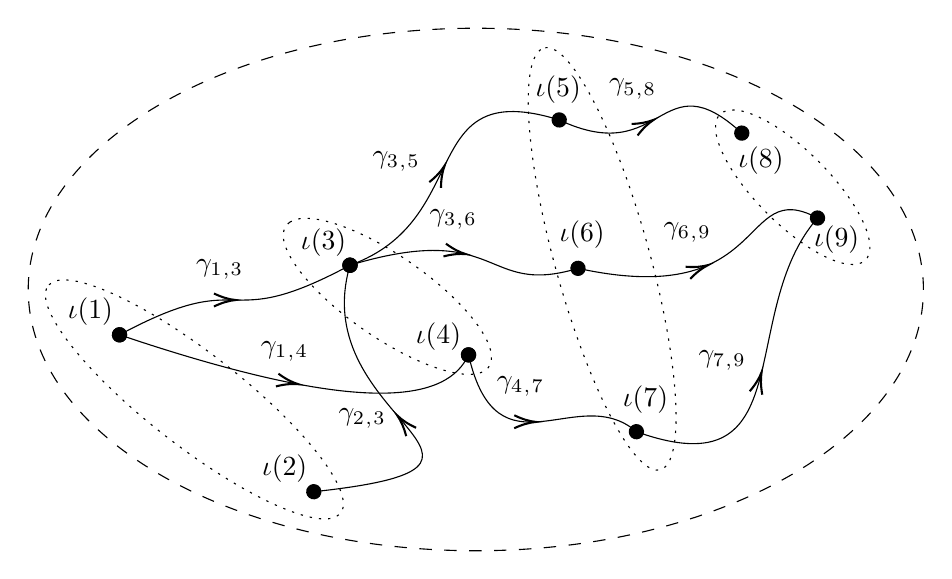
\begin{tikzpicture}[x=0.75pt,y=0.75pt,yscale=-0.95,xscale=0.95]
%uncomment if require: \path (0,281); %set diagram left start at 0, and has height of 281

%Shape: Ellipse [id:dp45216116111361904] 
\draw  [dash pattern={on 4.5pt off 4.5pt}] (6,138.5) .. controls (6,65.32) and (107.63,6) .. (233,6) .. controls (358.37,6) and (460,65.32) .. (460,138.5) .. controls (460,211.68) and (358.37,271) .. (233,271) .. controls (107.63,271) and (6,211.68) .. (6,138.5) -- cycle ;
%Curve Lines [id:da12378300176275903] 
\draw    (52.31,161.49) .. controls (119.1,125.59) and (102.4,162.09) .. (169.19,126.19) ;
\draw [shift={(169.19,126.19)}, rotate = 331.74] [color={rgb, 255:red, 0; green, 0; blue, 0 }  ][fill={rgb, 255:red, 0; green, 0; blue, 0 }  ][line width=0.75]      (0, 0) circle [x radius= 3.35, y radius= 3.35]   ;
\draw [shift={(111.13,143.84)}, rotate = 180.1] [color={rgb, 255:red, 0; green, 0; blue, 0 }  ][line width=0.75]    (10.93,-3.29) .. controls (6.95,-1.4) and (3.31,-0.3) .. (0,0) .. controls (3.31,0.3) and (6.95,1.4) .. (10.93,3.29)   ;
\draw [shift={(52.31,161.49)}, rotate = 331.74] [color={rgb, 255:red, 0; green, 0; blue, 0 }  ][fill={rgb, 255:red, 0; green, 0; blue, 0 }  ][line width=0.75]      (0, 0) circle [x radius= 3.35, y radius= 3.35]   ;
%Curve Lines [id:da3902364739215902] 
\draw    (169.19,126.19) .. controls (233.04,103.33) and (202.45,29.92) .. (275.29,52.51) ;
\draw [shift={(275.29,52.51)}, rotate = 17.23] [color={rgb, 255:red, 0; green, 0; blue, 0 }  ][fill={rgb, 255:red, 0; green, 0; blue, 0 }  ][line width=0.75]      (0, 0) circle [x radius= 3.35, y radius= 3.35]   ;
\draw [shift={(217.18,75.67)}, rotate = 476.11] [color={rgb, 255:red, 0; green, 0; blue, 0 }  ][line width=0.75]    (10.93,-3.29) .. controls (6.95,-1.4) and (3.31,-0.3) .. (0,0) .. controls (3.31,0.3) and (6.95,1.4) .. (10.93,3.29)   ;
\draw [shift={(169.19,126.19)}, rotate = 340.3] [color={rgb, 255:red, 0; green, 0; blue, 0 }  ][fill={rgb, 255:red, 0; green, 0; blue, 0 }  ][line width=0.75]      (0, 0) circle [x radius= 3.35, y radius= 3.35]   ;
%Curve Lines [id:da5125133831866234] 
\draw    (52.31,161.49) .. controls (178.45,204.05) and (218.84,194.46) .. (229.3,171.66) ;
\draw [shift={(229.3,171.66)}, rotate = 294.65] [color={rgb, 255:red, 0; green, 0; blue, 0 }  ][fill={rgb, 255:red, 0; green, 0; blue, 0 }  ][line width=0.75]      (0, 0) circle [x radius= 3.35, y radius= 3.35]   ;
\draw [shift={(142.99,186.54)}, rotate = 191.16] [color={rgb, 255:red, 0; green, 0; blue, 0 }  ][line width=0.75]    (10.93,-3.29) .. controls (6.95,-1.4) and (3.31,-0.3) .. (0,0) .. controls (3.31,0.3) and (6.95,1.4) .. (10.93,3.29)   ;
\draw [shift={(52.31,161.49)}, rotate = 18.65] [color={rgb, 255:red, 0; green, 0; blue, 0 }  ][fill={rgb, 255:red, 0; green, 0; blue, 0 }  ][line width=0.75]      (0, 0) circle [x radius= 3.35, y radius= 3.35]   ;
%Curve Lines [id:da9936282267570157] 
\draw    (150.83,241.06) .. controls (275.76,227.54) and (145.96,205.62) .. (169.19,126.19) ;
\draw [shift={(169.19,126.19)}, rotate = 286.3] [color={rgb, 255:red, 0; green, 0; blue, 0 }  ][fill={rgb, 255:red, 0; green, 0; blue, 0 }  ][line width=0.75]      (0, 0) circle [x radius= 3.35, y radius= 3.35]   ;
\draw [shift={(193.16,202.39)}, rotate = 409.89] [color={rgb, 255:red, 0; green, 0; blue, 0 }  ][line width=0.75]    (10.93,-3.29) .. controls (6.95,-1.4) and (3.31,-0.3) .. (0,0) .. controls (3.31,0.3) and (6.95,1.4) .. (10.93,3.29)   ;
\draw [shift={(150.83,241.06)}, rotate = 353.83] [color={rgb, 255:red, 0; green, 0; blue, 0 }  ][fill={rgb, 255:red, 0; green, 0; blue, 0 }  ][line width=0.75]      (0, 0) circle [x radius= 3.35, y radius= 3.35]   ;
%Curve Lines [id:da37329721640419344] 
\draw    (229.3,171.66) .. controls (243.97,235.64) and (284.76,184.82) .. (314.44,210.62) ;
\draw [shift={(314.44,210.62)}, rotate = 41] [color={rgb, 255:red, 0; green, 0; blue, 0 }  ][fill={rgb, 255:red, 0; green, 0; blue, 0 }  ][line width=0.75]      (0, 0) circle [x radius= 3.35, y radius= 3.35]   ;
\draw [shift={(263.43,205.67)}, rotate = 180.44] [color={rgb, 255:red, 0; green, 0; blue, 0 }  ][line width=0.75]    (10.93,-3.29) .. controls (6.95,-1.4) and (3.31,-0.3) .. (0,0) .. controls (3.31,0.3) and (6.95,1.4) .. (10.93,3.29)   ;
\draw [shift={(229.3,171.66)}, rotate = 77.09] [color={rgb, 255:red, 0; green, 0; blue, 0 }  ][fill={rgb, 255:red, 0; green, 0; blue, 0 }  ][line width=0.75]      (0, 0) circle [x radius= 3.35, y radius= 3.35]   ;
%Curve Lines [id:da6402293447536181] 
\draw    (169.19,126.19) .. controls (246.58,102.99) and (236.29,142.42) .. (284.82,127.77) ;
\draw [shift={(284.82,127.77)}, rotate = 343.19] [color={rgb, 255:red, 0; green, 0; blue, 0 }  ][fill={rgb, 255:red, 0; green, 0; blue, 0 }  ][line width=0.75]      (0, 0) circle [x radius= 3.35, y radius= 3.35]   ;
\draw [shift={(227.95,120.58)}, rotate = 190.98] [color={rgb, 255:red, 0; green, 0; blue, 0 }  ][line width=0.75]    (10.93,-3.29) .. controls (6.95,-1.4) and (3.31,-0.3) .. (0,0) .. controls (3.31,0.3) and (6.95,1.4) .. (10.93,3.29)   ;
%Curve Lines [id:da7275544623824886] 
\draw    (314.44,210.62) .. controls (399.23,240.98) and (364.55,150.12) .. (406.29,102.26) ;
\draw [shift={(406.29,102.26)}, rotate = 311.09] [color={rgb, 255:red, 0; green, 0; blue, 0 }  ][fill={rgb, 255:red, 0; green, 0; blue, 0 }  ][line width=0.75]      (0, 0) circle [x radius= 3.35, y radius= 3.35]   ;
\draw [shift={(377.94,180.41)}, rotate = 465.08] [color={rgb, 255:red, 0; green, 0; blue, 0 }  ][line width=0.75]    (10.93,-3.29) .. controls (6.95,-1.4) and (3.31,-0.3) .. (0,0) .. controls (3.31,0.3) and (6.95,1.4) .. (10.93,3.29)   ;
%Shape: Ellipse [id:dp21247917365246105] 
\draw  [color={rgb, 255:red, 0; green, 0; blue, 0 }  ,draw opacity=1 ][dash pattern={on 0.84pt off 2.51pt}] (16.54,136.11) .. controls (25.63,126.66) and (66.01,145.03) .. (106.72,177.14) .. controls (147.44,209.25) and (173.08,242.94) .. (163.99,252.39) .. controls (154.9,261.85) and (114.52,243.48) .. (73.81,211.37) .. controls (33.09,179.26) and (7.45,145.57) .. (16.54,136.11) -- cycle ;
%Curve Lines [id:da7880732583039812] 
\draw    (275.29,52.51) .. controls (328.72,77.63) and (326.15,20.9) .. (367.89,59.19) ;
\draw [shift={(367.89,59.19)}, rotate = 42.53] [color={rgb, 255:red, 0; green, 0; blue, 0 }  ][fill={rgb, 255:red, 0; green, 0; blue, 0 }  ][line width=0.75]      (0, 0) circle [x radius= 3.35, y radius= 3.35]   ;
\draw [shift={(323.24,52.43)}, rotate = 512.6] [color={rgb, 255:red, 0; green, 0; blue, 0 }  ][line width=0.75]    (10.93,-3.29) .. controls (6.95,-1.4) and (3.31,-0.3) .. (0,0) .. controls (3.31,0.3) and (6.95,1.4) .. (10.93,3.29)   ;
%Curve Lines [id:da726151739669847] 
\draw    (284.82,127.77) .. controls (383.33,149.3) and (366.22,80.72) .. (406.29,102.26) ;
\draw [shift={(350.78,126.12)}, rotate = 518.99] [color={rgb, 255:red, 0; green, 0; blue, 0 }  ][line width=0.75]    (10.93,-3.29) .. controls (6.95,-1.4) and (3.31,-0.3) .. (0,0) .. controls (3.31,0.3) and (6.95,1.4) .. (10.93,3.29)   ;
%Shape: Ellipse [id:dp20693904539608654] 
\draw  [color={rgb, 255:red, 0; green, 0; blue, 0 }  ,draw opacity=1 ][dash pattern={on 0.84pt off 2.51pt}] (138.62,104.37) .. controls (148.74,97.58) and (179.13,108.92) .. (206.48,129.69) .. controls (233.84,150.47) and (247.81,172.81) .. (237.69,179.59) .. controls (227.57,186.38) and (197.19,175.04) .. (169.83,154.27) .. controls (142.47,133.49) and (128.5,111.15) .. (138.62,104.37) -- cycle ;
%Shape: Ellipse [id:dp4442811176180146] 
\draw  [dash pattern={on 0.84pt off 2.51pt}] (268.26,15.88) .. controls (281.5,13.99) and (305.14,60.41) .. (321.05,119.55) .. controls (336.96,178.69) and (339.13,228.17) .. (325.89,230.05) .. controls (312.64,231.94) and (289.01,185.52) .. (273.09,126.38) .. controls (257.18,67.24) and (255.02,17.76) .. (268.26,15.88) -- cycle ;
%Shape: Ellipse [id:dp2537302094398456] 
\draw  [dash pattern={on 0.84pt off 2.51pt}] (358.5,48.46) .. controls (367.96,43.55) and (391.4,56.66) .. (410.84,77.74) .. controls (430.28,98.83) and (438.37,119.9) .. (428.91,124.82) .. controls (419.45,129.73) and (396.01,116.62) .. (376.57,95.54) .. controls (357.13,74.45) and (349.04,53.37) .. (358.5,48.46) -- cycle ;

% Text Node
\draw (50.31,158.09) node [anchor=south east] [inner sep=0.75pt]    {$\iota ( 1)$};
% Text Node
\draw (148.83,237.66) node [anchor=south east] [inner sep=0.75pt]    {$\iota ( 2)$};
% Text Node
\draw (168.57,122.92) node [anchor=south east] [inner sep=0.75pt]    {$\iota ( 3)$};
% Text Node
\draw (226.84,170.66) node [anchor=south east] [inner sep=0.75pt]    {$\iota ( 4)$};
% Text Node
\draw (262.03,45.25) node [anchor=south west] [inner sep=0.75pt]    {$\iota ( 5)$};
% Text Node
\draw (274.13,119.08) node [anchor=south west] [inner sep=0.75pt]    {$\iota ( 6)$};
% Text Node
\draw (306.28,202.6) node [anchor=south west] [inner sep=0.75pt]    {$\iota ( 7)$};
% Text Node
\draw (364.82,65) node [anchor=north west][inner sep=0.75pt]    {$\iota ( 8)$};
% Text Node
\draw (403.23,105) node [anchor=north west][inner sep=0.75pt]    {$\iota ( 9)$};
% Text Node
\draw (89.78,121.75) node [anchor=north west][inner sep=0.75pt]    {$\gamma _{1}{}_{,}{}_{3}$};
% Text Node
\draw (122.67,163.43) node [anchor=north west][inner sep=0.75pt]    {$\gamma _{1}{}_{,}{}_{4}$};
% Text Node
\draw (162.08,197.67) node [anchor=north west][inner sep=0.75pt]    {$\gamma _{2}{}_{,}{}_{3}$};
% Text Node
\draw (179.33,67.29) node [anchor=north west][inner sep=0.75pt]    {$\gamma _{3}{}_{,}{}_{5}$};
% Text Node
\draw (208.3,96.52) node [anchor=north west][inner sep=0.75pt]    {$\gamma _{3}{}_{,}{}_{6}$};
% Text Node
\draw (242.33,181.1) node [anchor=north west][inner sep=0.75pt]    {$\gamma _{4}{}_{,}{}_{7}$};
% Text Node
\draw (299.22,30.41) node [anchor=north west][inner sep=0.75pt]    {$\gamma _{5}{}_{,}{}_{8}$};
% Text Node
\draw (326.9,103.09) node [anchor=north west][inner sep=0.75pt]    {$\gamma _{6}{}_{,}{}_{9}$};
% Text Node
\draw (344.63,168.21) node [anchor=north west][inner sep=0.75pt]    {$\gamma _{7}{}_{,}{}_{9}$};


\end{tikzpicture}


\end{center}
\caption{A geometric graph}
\end{figure}
We notice that the same algebraic expression carries over:
\begin{align*}
        & (\gamma_{5, 8} \tensor (\gamma_{6, 9} \cwedge \gamma_{7, 9})) \\
  \circ & (\gamma_{3, 5} \tensor \gamma_{3, 6} \tensor \gamma_{4, 7}) \\
  \circ & ((\gamma_{3, 3} \cvee \gamma_{3, 3}) \tensor \gamma_{4, 4}) \\
  \circ & (\gamma_{3, 3} \tensor (\gamma_{4, 4} \boxtimes \gamma_{2, 3})) \\
  \circ & ((\gamma_{1, 3} \cvee \gamma_{1, 4}) \tensor \gamma_{2, 2})
\end{align*}
\end{exm}

At this point, we make a necessary observation. Consider geometric expression
graphs in a manifold equipped with an $A$--fibred bundle with connection. Then,
consider the expression of an expression graph realized in this manifold. If we
substitute the edges in the expression of the graph with the parallel transport
maps along the paths associated to the edges, we obtain a linear map from a
non-zero tensor power of $A$ to another such tensor power, given the graph has
at least one edge. However, there is no immediate way to obtain a map of the
form $\R \to A$ or $A \to \R$ in this method.

We recall that cobordisms $\varnothing \to S^1$ or
$S^1 \to \varnothing$ in $\Cob_2$ are given by composing cobordisms
$S^1 \to S^1$ with the following structures:
\[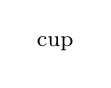
\begin{tikzpicture}[scale=0.5]
\cupcob{0, 2}
\node at (1.5, 0) (cuplbl) {{\footnotesize cup}};
\end{tikzpicture}
\qquad \qquad \qquad
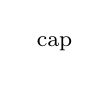
\begin{tikzpicture}[scale=0.5]
\capcob{3, 2}
\node at (1.5, 0) (caplbl) {{\footnotesize cap}};
\end{tikzpicture}\]
We would like analogous structures for expression graphs. We can use vertex
colouring to distinguish between copies of the empty manifold and copies of
$S^1$ in the result of the expression construction. So, we consider vertex
coloured expression graphs.
%Visually, loops
%attached to the source or target of an edge seem like possible candidates for
%these structures:
%\[\begin{tikzpicture}
%\node[circle, fill, inner sep=1.5pt] at (0, 0) (a) {};
%\node[circle, fill, inner sep=1.5pt] at (1, 0) (b) {};
%\draw[->] (a) [out=130, in=230, looseness=25] to (a);
%\midarrow{a}{b}
%\end{tikzpicture}
%\qquad \qquad \qquad
%\begin{tikzpicture}
%\node[circle, fill, inner sep=1.5pt] at (0, 0) (a) {};
%\node[circle, fill, inner sep=1.5pt] at (1, 0) (b) {};
%\draw[->] (b) [out=50, in=-50, looseness=25] to (b);
%\midarrow{a}{b}
%\end{tikzpicture}\]
%We will show that if we allow loops on vertices except for the ones which do not
%have any incoming or outgoing edges to begin with, then we can adapt the
%theory to this new setting.

%As a start, the expression construction algorithm is extended as follows:
%\begin{alg}
%Let $G$ be a graph where vertices, except for those without any edges from or to
%other vertices, can have loops. We then make the following modifications to $G$:
%\begin{enumerate}[(1)]
%\setlength{\itemsep}{0pt}
%
%\item Colour every vertex with a single colour -- say blue.
%
%\item If $u$ has no incoming edges except for a loop $(u, u)$ but has outgoing
%edges, then we add another copy $u'$ of $u$, color it green, add the edge
%$(u', u)$ and delete the loop $(u, u)$.
%\[\begin{tikzpicture}
%\node[circle, fill, inner sep=1.5pt, color=blue] at (0, 0) (a) {};
%\node[circle, fill, inner sep=1.5pt, color=blue] at (1, 0.5) (b1) {};
%\node[circle, fill, inner sep=1.5pt, color=blue] at (1, -0.5) (bn) {};
%\midarrow{a}{b1}
%\midarrow{a}{bn}
%\draw[->] (a) [out=130, in=230, looseness=15] to (a);
%\draw[loosely dotted, thick] (b1) -- (bn);
%\end{tikzpicture}
%\qquad
%\begin{tikzpicture}
%\node at (0, 0.5)   (TOP)     {};
%\node at (0, 0)   (TO)      {$\Longrightarrow$};
%\node at (0, -0.5)  (BOTTOM)  {};
%\end{tikzpicture}
%\qquad
%\begin{tikzpicture}
%\node[circle, fill, inner sep=1.5pt, color=green!55!black] at (0, 0) (a1) {};
%\node[circle, fill, inner sep=1.5pt, color=blue] at (1, 0) (a2) {};
%\node[circle, fill, inner sep=1.5pt, color=blue] at (2, 0.5) (b1) {};
%\node[circle, fill, inner sep=1.5pt, color=blue] at (2, -0.5) (bn) {};
%\midarrow{a1}{a2}
%\midarrow{a2}{b1}
%\midarrow{a2}{bn}
%\draw[loosely dotted, thick] (b1) -- (bn);
%\end{tikzpicture}\]
%
%\item If $u$ has incoming edges but no outgoing edges except for a loop
%$(u, u)$, then we add a green copy $u'$ of $u$ as before, add the edge $(u, u')$
%and delete the loop $(u, u)$.
%\[\begin{tikzpicture}
%\node[circle, fill, inner sep=1.5pt, color=blue] at (0, 0) (a) {};
%\node[circle, fill, inner sep=1.5pt, color=blue] at (-1, 0.5) (b1) {};
%\node[circle, fill, inner sep=1.5pt, color=blue] at (-1, -0.5) (bn) {};
%\midarrow{b1}{a}
%\midarrow{bn}{a}
%\draw[->] (a) [out=50, in=-50, looseness=15] to (a);
%\draw[loosely dotted, thick] (b1) -- (bn);
%\end{tikzpicture}
%\qquad
%\begin{tikzpicture}
%\node at (0, 0.5)   (TOP)     {};
%\node at (0, 0)   (TO)      {$\Longrightarrow$};
%\node at (0, -0.5)  (BOTTOM)  {};
%\end{tikzpicture}
%\qquad
%\begin{tikzpicture}
%\node[circle, fill, inner sep=1.5pt, color=green!55!black] at (0, 0) (a1) {};
%\node[circle, fill, inner sep=1.5pt, color=blue] at (-1, 0) (a2) {};
%\node[circle, fill, inner sep=1.5pt, color=blue] at (-2, 0.5) (b1) {};
%\node[circle, fill, inner sep=1.5pt, color=blue] at (-2, -0.5) (bn) {};
%\midarrow{a2}{a1}
%\midarrow{b1}{a2}
%\midarrow{bn}{a2}
%\draw[loosely dotted, thick] (b1) -- (bn);
%\end{tikzpicture}\]
%
%\item If $u$ has both incoming and outgoing edges along with a loop $(u, u)$,
%we replace the loop with a path $u, u', u''$, where $u'$ is a green copy of $u$
%and $u''$ is another blue copy of $u$.
%\[\begin{tikzpicture}
%\node[circle, fill, inner sep=1.5pt, color=blue] at (0, 0) (a) {};
%\node[circle, fill, inner sep=1.5pt, color=blue] at (1, 0.35) (b1) {};
%\node[circle, fill, inner sep=1.5pt, color=blue] at (1, -0.35) (bn) {};
%\node[circle, fill, inner sep=1.5pt, color=blue] at (-1, 0.35) (c1) {};
%\node[circle, fill, inner sep=1.5pt, color=blue] at (-1, -0.35) (cn) {};
%\midarrow{a}{b1}
%\midarrow{a}{bn}
%\draw[->] (a) [out=60, in=120, looseness=15] to (a);
%\midarrow{c1}{a}
%\midarrow{cn}{a}
%\draw[loosely dotted, thick] (b1) -- (bn);
%\draw[loosely dotted, thick] (c1) -- (cn);
%\end{tikzpicture}
%\qquad
%\begin{tikzpicture}
%\node at (0, 0.35)   (TOP)     {};
%\node at (0, 0)   (TO)      {$\Longrightarrow$};
%\node at (0, -0.35)  (BOTTOM)  {};
%\end{tikzpicture}
%\qquad
%\begin{tikzpicture}
%\node[circle, fill, inner sep=1.5pt, color=blue] at (-1, 0) (a1) {};
%\node[circle, fill, inner sep=1.5pt, color=green!55!black] at (0, 0) (a2) {};
%\node[circle, fill, inner sep=1.5pt, color=blue] at (1, 0) (a3) {};
%\node[circle, fill, inner sep=1.5pt, color=blue] at (2, 0.35) (b1) {};
%\node[circle, fill, inner sep=1.5pt, color=blue] at (2, -0.35) (bn) {};
%\node[circle, fill, inner sep=1.5pt, color=blue] at (-2, 0.35) (c1) {};
%\node[circle, fill, inner sep=1.5pt, color=blue] at (-2, -0.35) (cn) {};
%\midarrow{a3}{b1}
%\midarrow{a3}{bn}
%\midarrow{c1}{a1}
%\midarrow{cn}{a1}
%\midarrow{a1}{a2}
%\midarrow{a2}{a3}
%\draw[loosely dotted, thick] (b1) -- (bn);
%\draw[loosely dotted, thick] (c1) -- (cn);
%\end{tikzpicture}\]
%
%\item If $G$ is a disjoint union $\coprod_i G_i$ and some $G_i = \varnothing$,
%we replace $G_i$ with an edge $(u_{G_i}, v_{G_i})$, where both the vertices are
%green:
%\[\begin{tikzpicture}
%\node at (0, 0) (a) {$\varnothing$};
%\end{tikzpicture}
%\qquad
%\begin{tikzpicture}
%\node at (0, 0)   (TO)      {$\Longrightarrow$};
%\end{tikzpicture}
%\qquad
%\begin{tikzpicture}
%\node[circle, fill, inner sep=1.5pt, color=green!55!black] at (0, 0) (a1) {};
%\node[circle, fill, inner sep=1.5pt, color=green!55!black] at (2, 0) (a3) {};
%\midarrow{a1}{a3}
%\end{tikzpicture}\]
%\begin{rmk}
%This is a case we ignored in the first expression construction aglorithm -- we
%did so for simplicity. We handle this now because we now have a way to deal with
%empty sources and targets.
%\end{rmk}
%
%\item We apply the steps of the first expression construction algorithm with
%copied vertices having the same colour as the original.
%
%\item We then identify green vertices with the empty manifold and obtain our
%expression from the identification of the graph in its final state with some
%cobordism in $\Cob_2$.
%
%\end{enumerate}
%\end{alg}

%Disjoint unions are easily adapted as well. However, we will change our
%definitions of source and target expression graphs since we will now interpret
%looped vertices as cobordisms of the empty manifold. We first adapt expression
%graphs to include loops.

\begin{defn}[Pretransport Graph]
A pretransport graph is an expression graph $G$ with a colour function
$V(G) \to \set{{\color{green!55!black}\text{green}},
{\color{blue!55!black}\text{blue}}}$ (with no constraints on adjacency of
vertices).
\end{defn}

\begin{defn}[Pretransport Homomorphism]
A pretransport homomorphism is a colour-preserving expression homomorphism.
\end{defn}

%\begin{rmk}
%We note that pretransport homomorphisms, being graph homomorphisms must preserve
%loops.
%\end{rmk}

From \ref{cor:expiso_unique}, it is immediate that:

\begin{cor}
Pretransport isomorphisms are unique.
\end{cor}

We now redefine the source and target of a pretransport graph so that
constructions like expressions and gluing can be adapted to this new setting
where we allow empty graphs to be sources and targets.

\begin{defn}
Let $G$ be a pretransport graph with $s_1, \dots, s_n$ the ordering of the
source vertices of its underlying expression graph and $t_1, \dots, t_m$ the
ordering of the target vertices thereof. Let $s_{i_1}, \dots, s_{i_p}$ be the
green source vertices and $t_{j_1}, \dots t_{j_q}$ be the green target vertices
in $G$. Then, the source of $G$ is defined to be the expression graph
\[
  S(G) := \set{s_1, \dots, s_{i_1 - 1}}
       \amalg \varnothing
       \amalg \set{s_{i_1 + 1}, \dots, s_{i_2}}
       \amalg \varnothing
       \amalg \cdots
       \amalg \varnothing
       \amalg \set{s_{i_p + 1}, \dots, s_{n}}
\]
The target of $G$ is defined to be the expression graph
\[
  T(G) := \set{t_{1}, \dots, t_{j_1 - 1}}
       \amalg \varnothing
       \amalg \set{t_{j_1 + 1}, \dots, t_{j_2}}
       \amalg \varnothing
       \amalg \cdots
       \amalg \varnothing
       \amalg \set{t_{j_q + 1}, \dots, t_{m}}
\]
\end{defn}

\begin{defn}
Gluing of expression graphs extends to gluing of pretransport graphs if we
consider pretransport isomorphisms instead of expression isomorphisms. More
precisely, for pretransport graphs $G$ and $H$, if $S(H) \cong T(G)$, then the
gluing is exactly the same as for expression graphs except for positions where
we have instances of $\varnothing$. For this, we have the following cases:
\begin{enmrt}
\li $H$ and $G$ both have green vertices at that position: we glue them
as usual.
\li $H$ has a green vertex but $G$ has $\varnothing$: we simply forget
that $G$ has $\varnothing$.
\li $H$ has $\varnothing$ but $G$ has a green vertex: we forget the copy
of $\varnothing$
\li $H$ and $G$ both have copies of $\varnothing$: we keep a single copy
of $\varnothing$
\end{enmrt}
\end{defn}

\begin{defn}[Expression Construction]
The expression of a pretransport graph $G$ is obtained by running the expression
construction on $G$ by forgetting colours and then identifying green vertices
with the empty manifold in the resulting cobordism in $\Cob_2$.
\end{defn}

We then consider the class of graphs that will yield our desired linear maps.

\begin{defn}[Transport Graph]
We call a geometric pretransport graph a transport graph.
\end{defn}

\begin{defn}[Geometric Homomorphism]
Let $G$ and $H$ be graphs in manifolds $M$ and $N$ with geometric realizations
$\gamma^G$ and $\gamma^H$ respectively, then a homomorphism $h : G \to H$
equipped with a smooth map $f : M \to N$ making the following diagram commute is
called a geometric homomorphism:
\[\begin{tikzpicture}[baseline=(a).base]
\node[scale=\diagscale] (a) at (0, 0){
\begin{tikzcd}
E(G) \ar[d, "\gamma^G" left] \ar[r, "h" above] &
E(H) \ar[d, "\gamma^H" right] \\
C^0(I, M) \ar[r, "f_*" below] &
C^0(I, N)
\end{tikzcd}
};
\end{tikzpicture}\]
where $f_*$ is the post-composition map $g \mapsto f \circ g$, and the
homomorphism $h$ is viewed as the function it induces on edge sets.
\end{defn}

\begin{defn}[Transport Homomorphism]
A geometric pretransport homomorphism is called a transport homomorphism.
\end{defn}

Pasting commutative squares as the one above along the $\gamma$ sides, we
observe that geometric homomorphisms compose associatively. Taking
$h$ and $f$ as the identity maps yields an identity morphism of geometric
graphs. Similarly, transport homomorphism also compose associatively and have
units. Furthermore, transport graphs inherit the disjoint union from their
underlying expression graphs and manifolds. For their gluing, we require a
notion of gluing geometric realizations.

We first observe that if $G$ and $H$ are transport graphs with a transport
isomorphism $S(H) \to T(G)$, it is unique by \ref{cor:expiso_unique}, since
there is only one map of path sets -- the empty map which always makes the
rquired diagram commute. We then have the following basic fact.

\begin{cor}
Let $G$ and $H$ be transport graphs realized in manifolds
$M$ and $N$ with geometric realizations $\gamma^G$ and
$\gamma^H$ respectively such that $\psi_{G, H} : S(H) \to T(G)$ is a unique
pretransport homomorphism, and $M$ and $N$ are ``smoothly gluable'' at some
part. Then, there exists a geometric realization
\[
  \gamma^H * \gamma^G : E(H * G) \to C^0(I, N * M)
\]
of the pretransport graph $H * G$ in $N * M$.
\end{cor}
\begin{proof}
We can define $\gamma^H * \gamma^G$ piecewise since the gluing site has no
edges.
\end{proof}

\begin{defn}[Gluing Transport Graphs]
For transport graphs $(G, \gamma^G)$ and $(H, \gamma^H)$ with $S(H) \cong T(G)$
with a transport homomorphism, we define their gluing in the obvious way:
\[
  (H, \gamma^H) * (G, \gamma^G) := (H * G, \gamma^H * \gamma^G)
\]
\end{defn}

This is enough structure to develop a simple system for doing algebra using
paths on a manifold. In particular, it yields at least two monoidal double
categories of transport graphs realized in manifolds. We develop one of these
notions of TQFTs next.
\TODO{I am not sure if it is appropriate call this a notion of TQFTs.}




\subsection{Single Manifold TQFT}\label{subsec:sing_man_tqft}

Notice that the theory we developed so far transfers verbatim from the smooth
setting to the setting of complex bundles in that we can replace all instances
of $\R$ with $\C$, smooth bundles and $\R$--linear connections with smooth
manifolds, complex bundles and $\C$--linear connections on complex bundles
respectively. From this point onwards, when we say manifold, bundle, connection,
etc., we will mean these in either of the two settings. We will write $\K$ to
mean either of $\R$ or $\C$. With this convention, we consider the following
data for a monoidal double category:

\begin{enmrt}
\li Object category: objects are totally ordered, $2$--coloured, finite sets;
morphisms are order-preserving, colour-preserving (unique) bijections
$V \stackrel{!}{\longleftrightarrow} V'$

\li Morphism category: objects (horizontal $1$--morphisms) are transport graphs
$(G, \gamma)$, where for a fixed manifold $M$, a fixed bundle $\pi : E \to M$,
and a fixed connection $\nabla$ on $\pi$, $G$ is a pretransport graph with
$\gamma$ a geometric realization of $G$ in $M$; morphisms are tuples
\[
  (f_0, f_1, h) : (G_1, \gamma^1) \to (G_2, \gamma^2)
\]
where $(f_0, f_1)$ is an automorphism of the connection $\nabla$ and
$(f_0, h)$ is a transport isomorphism $(G_1, \gamma^1) \to (G_2, \gamma^2)$
\footnote{It is possible that this condition forces $(f_0, f_1) = (\id, \id)$.}

\li Source functor: $S : G \mapsto S(G)$; for a $2$--morphism $(f_0, f_1, h)$,
$S(f_0, f_1, h)$ is the unique order-preserving bijection
$S(\dom h) \to S(\codom h)$

\li Target functor: $T : G \mapsto T(G)$, defined similarly as $S$

\li Unit functor: $U : V \mapsto V$; $U : f \mapsto f$ -- each finite,
totally-ordered, $2$--coloured set is a transport graph with no edges and
order- and colour- preserving bijections between finite sets are unique
transport isomorphisms

\li Horizontal composition:
$(G_2, \gamma^2) * (G_1, \gamma^1) = (G_2 * G_1, \gamma^2 * \gamma^1)$

\li Horizontal associators: inherited from the categories of sets and manifolds

\li Horizontal unitors: inherited like associators

\li Monoidal product: disjoint union

\li Monoidal unit: empty set for object category, empty graph for morphism
category
\end{enmrt}

\begin{defn}[Double Category of Transport Graphs in a Manifold]
The above data defines the double category of transport graphs in $M$ and we
denote it as $\TG(M)$. We denote the object category as $\TG(M)_0$ and the
morphism category as $\TG(M)_1$.
\end{defn}

We then consider a double functor defined as follows.

\begin{defn}[Parallel Field Theory over a Manifold]\label{defn:sing_man_tqft}
For a finite, totally-ordered, $2$--coloured set
$V = \set{v_1, \dots, v_n}$ in $\TG(M)_0$, we set
\[
  F(V) := \bigotimes_{i = 1}^{n} c(v_i)
\]
where $c(v) = A$ if $v$ is blue and $c(v) = \K$ if $v$ is green,
for some $\K$--algebra $A$.

For every unique order- and colour-preserving bijection $f : V \to V'$ in
$\TG(M)_0$, we set $F(f) := \id_{F(V)} = \id_{F(V')}$.

For a transport graph $(G, \gamma)$ in $M$ -- an object in $\TG(M)_1$ -- and an
edge $(u, v) \in G$, we denote $\nabla^{\gamma_{u, v}}$ to be the linear map
$A \to A$ obtained by parallel transport along $\gamma_{u, v}$, with respect to
$\nabla$. Fixing some element $a_{u, v} \in A$, we then define:
\[
  F(u, v) := \begin{cases}
    \id_A
      & u = v \text{ is blue} \\
    \id_{\K} % 1 \mapsto \text{trace}\br{\nabla^{\gamma_{u, v}}(a_{u, v})}
      & u \text{ is green and } v \text{ is green} \\
    \nabla^{\gamma_{u, v}}
      & u \text{ is blue and } v \text{ is blue} \\
    1 \mapsto \nabla^{\gamma_{u, v}}(a_{u, v})
      & u \text{ is green and } v \text{ is blue} \\
    \text{trace} \circ \nabla^{\gamma_{u, v}}
      & u \text{ is blue and } v \text{ is green}
  \end{cases}
\]
We then obtain a linear map:
\[
  F(G, \gamma) := \Exp{G}[F(u, v)]
               :  F(S(G)) \to F(T(G))
\]
For a $2$--morphism
$(f_0, f_1, h) : (G_1, \gamma_1) \to (G_2, \gamma_2)$ in $\TG(M)_1$, we consider
the path $(r_t, s_t)$ in the isomorphism group of the connection $\nabla$ such
that $(r_0, s_0) = (\id_M, \id_E)$ and $(r_1, s_1) = (f_0, f_1)$. We then have a
smoothly varying family of functions $s_t\gamma : E(G) \to C^0(I, M)$
where $(s_t\gamma)_{u, v} = s_t \circ \gamma_{u, v}$. This yields a smoothly
varying family of linear maps, which we write as:
\[
  F(f_0, f_1, h) := \Exp{G}[s_t\gamma]
    : F(S(G)) \to F(T(G)), t \in [0, 1]
\]
We call $F$ a parallel field theory on $M$.
\end{defn}

\begin{rmk}\label{rmk:any_vect_space}
We note that so far we have considered $\cwedge$ and $\cvee$ to mean the product
and its dual for some algebra $A$. This is not strictly necessary. We could, in
principle, choose, for each instance of $\cwedge$ in an expression of a
transport graph, a distinct map $A \tensor A \to A$ when defining a parallel
field theory as above, as long as it does not disturb the monoidal double
functoriality of $F$. In fact, we could replace $A$ with an arbitrary vector
space $V$ and work with arbitrary linear maps $V \tensor V \to V$ and
$V \to V \tensor V$ in replacing $\cwedge$ and $\cvee$ in expressions arising
from transport graphs.
\end{rmk}

We note that the definition of $F$ does not specify the codomain. We will define
the codomain double category in the next section along with a notion of TQFTs
based on transport graphs in cobordisms equipped with connections.

We also note that there is some redundancy in this setup. The empty graph, the
single green vertex and paths with only green vertices are not the same
horizontal $1$--morphism but they are all morphisms
$\varnothing \to \varnothing$ and map to the identity morphism of $\K$ under
$F$. This differs from $\Cob_2$ and $2\Thick$ in that there are unique
morphisms $\varnothing \to \varnothing$ in these categories as well as their
corresponding double categories that map to the identity morphism of $\K$ under
a usual TQFT.



\end{document}

